\chapter{Risultati}
Questo capitolo ha l'obiettivo di discutere i risultati sperimentali ottenuti con l'esecuzione
dell'algoritmo del simplesso e dell'algoritmo di Frank-Wolfe su istanze del rilassamento lineare del set-covering.

\section{Prove sperimentali}
Per valutare l'efficienza e l'applicabilità dell'algoritmo di Frank-Wolfe abbiamo effettuato varie prove sperimentali su
numerose istanze, variando la dimensione e la sparsità della matrice di riferimento. Inoltre, per ogni coppia di valori
che identificano dimensione e sparsità abbiamo ripetuto gli esperimenti su molteplici istanze, con l'obiettivo di
ottenere risultati più accurati. Infine abbiamo calcolato la media e la deviazione standard di questi risultati, in modo
da poterli riassumere utilizzando opportuni grafici.

Inizialmente abbiamo condotto degli esperimenti per studiare la qualità della soluzione prodotta dall'algoritmo di
Frank-Wolfe, confrontandola con il valore ottimo ottenuto attraverso l'algoritmo del simplesso.

Successivamente abbiamo svolto delle prove per confrontare i tempi di esecuzione dei due algoritmi, con l'obiettivo di
capire se è possibile utilizzare l'algoritmo di Frank-Wolfe per trovare una limitazione ragionevole al valore ottimo in
un tempo molto ridotto.

Nello svolgimento degli esperimenti abbiamo scelto valori di sparsità particolarmente alti, in accordo con il fatto che
i problemi di set-covering sono caratterizzati da matrici generalmente molto sparse.

\newpage
\section{Qualità delle soluzioni}
Procediamo ora con l'esecuzione dei due algoritmi per confrontare le limitazioni prodotte dall'algoritmo di Frank-Wolfe
con il valore ottimo trovato dall'algoritmo del simplesso. In questo esperimento non ci preoccupiamo di
limitare il numero delle iterazioni, e quindi il tempo di esecuzione di Frank-Wolfe, poiché l'obiettivo è solamente quello
di determinare la qualità delle limitazioni prodotte.

\subsection{Dimensione della matrice di riferimento}
Iniziamo considerando istanze di dimensioni differenti. In questo contesto ci limiteremo ad analizzare gli aspetti che
riguardano il numero di elementi della matrice di riferimento, ignorando tutti gli altri parametri che verranno
analizzati singolarmente nel seguito. I risultati sono riassunti nei grafici della Figura \ref{fig:bysize} e riportati
nella Tabella \ref{table:bysize}.
\begin{figure}[ht]
    \centering
    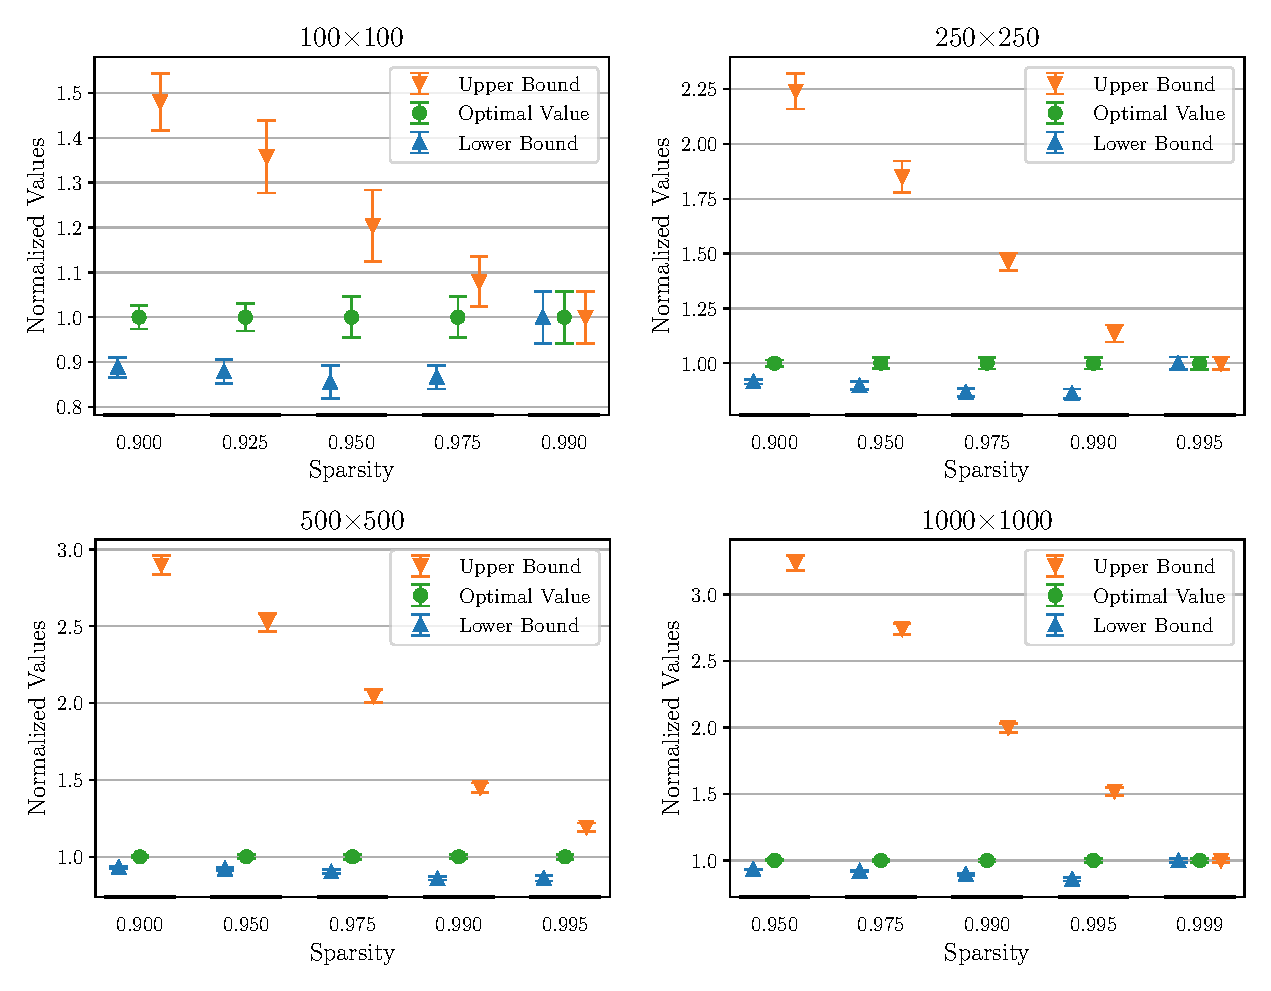
\includegraphics[width=\textwidth]{assets/figures/size.pdf}
    \caption{Qualità delle limitazioni prodotte dall'algoritmo di Frank-Wolfe al variare della sparsità e del numero di elementi della
    matrice di riferimento delle istanze.}
    \label{fig:bysize}
\end{figure}

\begin{table}[!ht]
    \centering
    \vspace*{45pt}
    \begin{tabularx}{355.3615pt}{cccc}
        \toprule
        \text{\alt Matrice} & \text{\alt Sparsità} & \text{\alt Limitazione Inferiore} & \text{\alt Limitazione Superiore} \\
        \midrule
        \( 100\times 100 \)
        & 0.900 & 0.888 & 1.480 \\
        & 0.925 & 0.879 & 1.358 \\
        & 0.950 & 0.855 & 1.204 \\
        & 0.975 & 0.867 & 1.080 \\
        & 0.990 & 1.000 & 1.000 \\
        \midrule
        \( 250\times 250 \)
        & 0.900 & 0.916 & 2.241 \\
        & 0.950 & 0.899 & 1.850 \\
        & 0.975 & 0.867 & 1.462 \\
        & 0.990 & 0.861 & 1.136 \\
        & 0.995 & 1.000 & 1.000 \\
        \midrule
        \( 500\times 500 \)
        & 0.900 & 0.931 & 2.898 \\
        & 0.950 & 0.920 & 2.525 \\
        & 0.975 & 0.903 & 2.047 \\
        & 0.990 & 0.859 & 1.449 \\
        & 0.995 & 0.860 & 1.191 \\
        \midrule
        \( 1000\times 1000 \)
        & 0.950 & 0.932 & 3.237 \\
        & 0.975 & 0.920 & 2.741 \\
        & 0.990 & 0.896 & 1.998 \\
        & 0.995 & 0.859 & 1.519 \\
        & 0.999 & 1.000 & 1.000 \\
        \bottomrule
    \end{tabularx}
    \caption{Valori delle limitazioni prodotte da Frank-Wolfe, normalizzati rispetto al valore ottimo fornito dal
    simplesso, al variare della dimensione delle matrici di riferimento.}
    \label{table:bysize}
\end{table}

Osserviamo che, a parità di sparsità, l'aumentare del numero di elementi della matrice di riferimento è indicatore di un
peggioramento nella qualità della limitazione superiore per tutte le istanze che abbiamo considerato. Il comportamento
della limitazione inferiore è invece più irregolare. In particolare, quando il valore di sparsità è abbastanza basso le
limitazioni inferiori migliori si ottengono per matrici di dimensione maggiore. Al contrario, per valori di sparsità
sufficientemente elevati avere matrici di dimensione minore permette di ottenere limitazioni inferiori di qualità
maggiore e talvolta di chiudere sul valore ottimo.

Per le matrici di dimensione fissata, l'aumento di sparsità determina un miglioramento della limitazione superiore ma
non della limitazione inferiore, che ha un comportamento più irregolare.

In tutti i casi, le variazioni delle limitazioni superiori sono più marcate rispetto alle variazioni delle limitazioni
inferiori, che rimangono invece molto più stabili.

\subsection{Forma della matrice di riferimento}
Procediamo ora a considerare istanze caratterizzate da matrici di riferimento di forme differenti, con l'obiettivo di
capire come la forma della matrice influenza la qualità delle limitazioni prodotte dall'algoritmo di Frank-Wolfe. In
particolare, faremo riferimento istanze caratterizzate da matrici di riferimento in cui il numero delle righe e delle
colonne è sbilanciato da un parte oppure dall'altra, come accade nella maggior parte delle istanze relative a problemi
di set-covering.

I risultati per istanze di taglia piccola e media, caratterizzate da matrici di riferimento con lo stesso numero di
elementi ma forma differente, sono riassunti nei grafici della Figura \ref{fig:shape1} e riportati nella Tabella
\ref{table:shape1}.

\begin{figure}[ht]
    \centering
    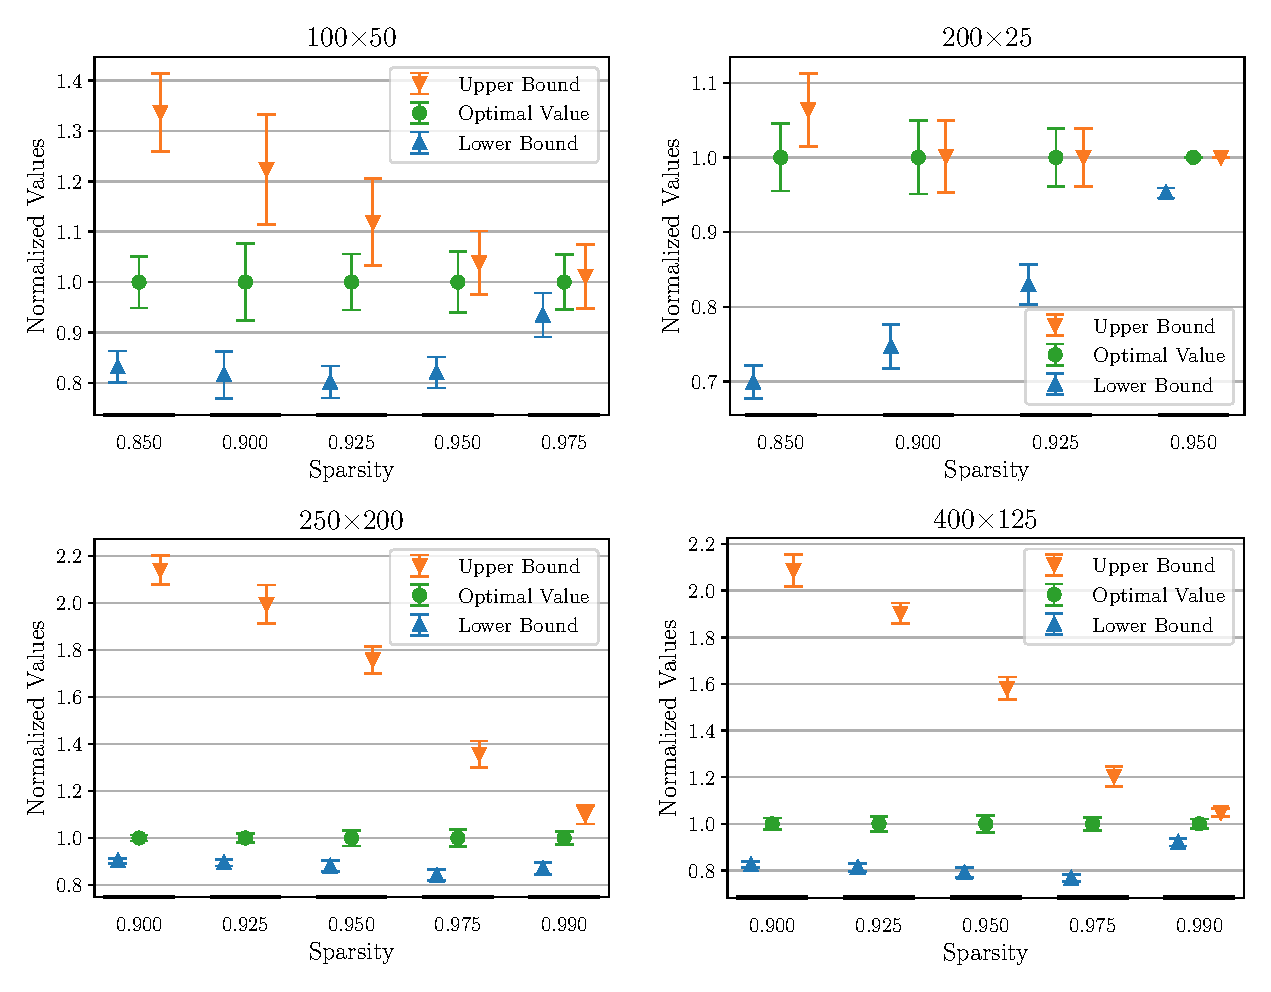
\includegraphics[width=\textwidth]{assets/figures/shape1.pdf}
    \caption{Qualità delle limitazioni prodotte dall’algoritmo di Frank-Wolfe al variare della sparsità e della forma
    della matrice di riferimento di istanze piccole e medie.}
    \label{fig:shape1}
\end{figure}

Se consideriamo le singole istanze, notiamo ancora una volta che l'aumento di sparsità è indicatore di un miglioramento
della limitazione superiore ma non della limitazione inferiore, che ha un comportamento più irregolare.

\begin{table}[!ht]
    \centering
    \vspace*{40pt}
    \begin{tabularx}{343.61162pt}{cccc}
        \toprule
        \text{\alt Matrice} & \text{\alt Sparsità} & \text{\alt Limitazione Inferiore} & \text{\alt Limitazione Superiore} \\
        \midrule
        \( 100\times 50 \)
        & 0.850 & 0.832 & 1.337 \\
        & 0.900 & 0.816 & 1.224 \\
        & 0.925 & 0.802 & 1.119 \\
        & 0.950 & 0.821 & 1.038 \\
        & 0.975 & 0.935 & 1.011 \\
        \midrule
        \( 200\times 25 \)
        & 0.850 & 0.699 & 1.063 \\
        & 0.900 & 0.747 & 1.001 \\
        & 0.925 & 0.830 & 1.000 \\
        & 0.950 & 0.952 & 1.000 \\
        \midrule
        \( 250\times 200 \)
        & 0.900 & 0.904 & 2.139 \\
        & 0.925 & 0.895 & 1.993 \\
        & 0.950 & 0.881 & 1.757 \\
        & 0.975 & 0.842 & 1.357 \\
        & 0.990 & 0.871 & 1.098 \\
        \midrule
        \( 400\times 125 \)
        & 0.900 & 0.825 & 2.086 \\
        & 0.925 & 0.814 & 1.903 \\
        & 0.950 & 0.790 & 1.582 \\
        & 0.975 & 0.768 & 1.203 \\
        & 0.990 & 0.921 & 1.048 \\
        \bottomrule
    \end{tabularx}
    \caption{Valori delle limitazioni prodotte da Frank-Wolfe, normalizzati rispetto al valore ottimo fornito dal
    simplesso, al variare della forma della matrice di riferimento di istanze piccole e medie.}
    \label{table:shape1}
\end{table}

Osserviamo che, a parità di sparsità, la forma della matrice di riferimento influenza la qualità delle limitazioni
prodotte dall'algoritmo di Frank-Wolfe, anche se il numero degli elementi rimane lo stesso. In particolare, le
limitazioni superiori migliori si ottengono per le istanze caratterizzate da un numero di variabili inferiori. Ad
esempio, le matrici \( 200\times 25 \) producono limitazioni superiori migliori rispetto alle matrici  \( 100\times 50
\), a prescindere dalla sparsità della matrice di riferimento. Lo stesso vale per le matrici \( 400\times 125 \), che
producono limitazioni superiori migliori rispetto alle matrici \( 250\times 200 \).

Le limitazioni inferiori migliori si ottengono con le istanze caratterizzate da un numero di variabili maggiore, quando
i valori di sparsità sono abbastanza bassi, e con le istanze caratterizzate da un numero di variabili minore, quando i
valori di sparsità sono sufficientemente elevati.

Considerando istanze di taglia grande, otteniamo i risultati riassunti nella Figura \ref{fig:shape2} e riportati nella
Tabella \ref{table:shape2}.

\begin{figure}[ht]
    \centering
    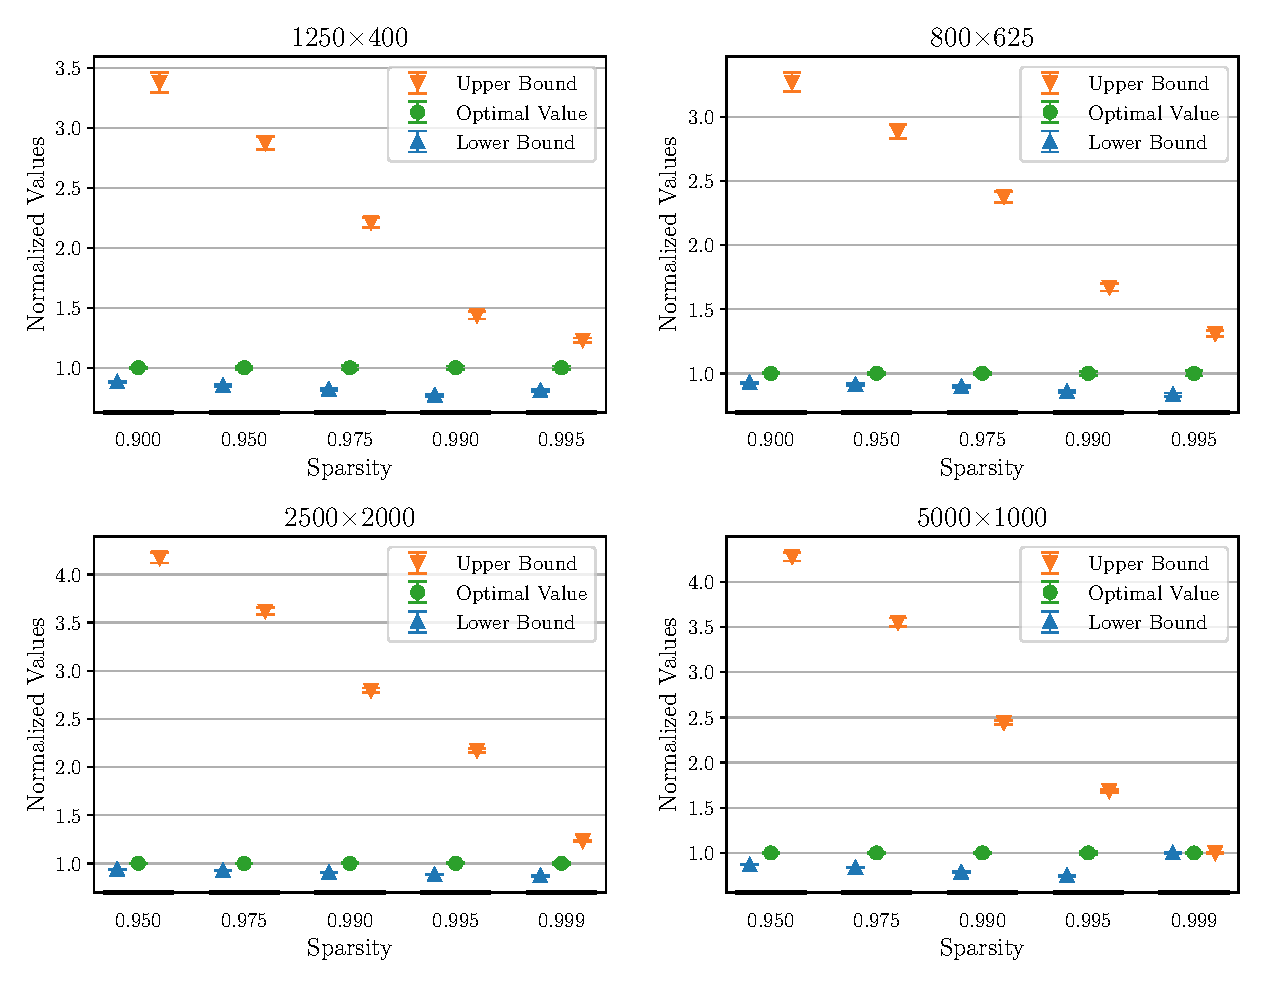
\includegraphics[width=\textwidth]{assets/figures/shape2.pdf}
    \caption{Qualità delle limitazioni prodotte dall’algoritmo di Frank-Wolfe al variare della sparsità e della forma
    della matrice di riferimento di istanze grandi.}
    \label{fig:shape2}
\end{figure}

Notiamo che il comportamento delle limitazioni superiori è lo stesso che abbiamo ottenuto per matrici più piccole, ma è
meno evidente e si verifica solamente per valori di sparsità più elevati. Ad esempio, le matrici
\(
    1250\times 400
\)
producono limitazioni superiori migliori rispetto alle matrici
\(
    800\times 625
\)
quando la sparsità è maggiore o uguale a 0.950. Similmente, le matrici
\(
    5000\times 1000
\)
producono limitazioni superiori migliori rispetto alle matrici \( 2500\times 2000 \), ma solo per valori di sparsità
maggiori o uguali a 0.975.

Le limitazioni inferiori hanno un comportamento differente rispetto a prima. Ad esempio, le matrici \( 800\times 625 \)
producono limitazioni inferiori migliori rispetto alle matrici
\(
    1250\times 400,
\)
a prescindere dal valore di sparsità. Similmente, le matrici \( 2500\times 2000 \) producono limitazioni inferiori
migliori rispetto alle matrici \( 5000\times 1000 \), ma solo per valori di sparsità minori o uguali a 0.995.

La diversità nel comportamento delle limitazioni inferiori per matrici grandi rispetto a matrici più piccole suggerisce
che la dimensione e la sparsità non costituiscono fattori così determinanti in questo caso.

\begin{table}[!ht]
    \centering
    \vspace*{40pt}
    \begin{tabularx}{355.3615pt}{cccc}
        \toprule
        \text{\alt Matrice} & \text{\alt Sparsità} & \text{\alt Limitazione Inferiore} & \text{\alt Limitazione Superiore} \\
        \midrule
        \( 800\times 625 \)
        & 0.900 & 0.928 & 3.270 \\
        & 0.950 & 0.912 & 2.884 \\
        & 0.975 & 0.897 & 2.377 \\
        & 0.990 & 0.858 & 1.671 \\
        & 0.995 & 0.835 & 1.310 \\
        \midrule
        \( 1250\times 400 \)
        & 0.900 & 0.882 & 3.378 \\
        & 0.950 & 0.853 & 2.874 \\
        & 0.975 & 0.820 & 2.211 \\
        & 0.990 & 0.771 & 1.438 \\
        & 0.995 & 0.810 & 1.230 \\
        \midrule
        \( 2500\times 2000 \)
        & 0.950 & 0.939 & 4.173 \\
        & 0.975 & 0.926 & 3.620 \\
        & 0.990 & 0.905 & 2.799 \\
        & 0.995 & 0.886 & 2.175 \\
        & 0.999 & 0.871 & 1.233 \\
        \midrule
        \( 5000\times 1000 \)
        & 0.950 & 0.869 & 4.275 \\
        & 0.975 & 0.836 & 3.551 \\
        & 0.990 & 0.786 & 2.440 \\
        & 0.995 & 0.748 & 1.686 \\
        & 0.999 & 1.000 & 1.000 \\
        \bottomrule
    \end{tabularx}
    \caption{Valori delle limitazioni prodotte da Frank-Wolfe, normalizzati rispetto al valore ottimo fornito dal
    simplesso, al variare della forma della matrice di riferimento di istanze grandi.}
    \label{table:shape2}
\end{table}

Il comportamento delle limitazioni inferiori non sembra dipendere tanto dal numero degli elementi della
matrice di riferimento, ma quanto più dal bilanciamento di variabili e vincoli. In altre parole, sperimentalmente si
osserva che la qualità delle limitazioni inferiori prodotte dall'algoritmo di Frank-Wolfe è migliore per le istanze
caratterizzate da matrici di riferimento bilanciate, relativamente al numero delle righe e delle colonne. Per confermare
questa ipotesi, abbiamo utilizzato delle ulteriori istanze. I risultati sono riassunti nei grafici della Figura
\ref{fig:shape3} e riportati nella Tabella \ref{table:shape3}.

\begin{figure}[ht]
    \centering
    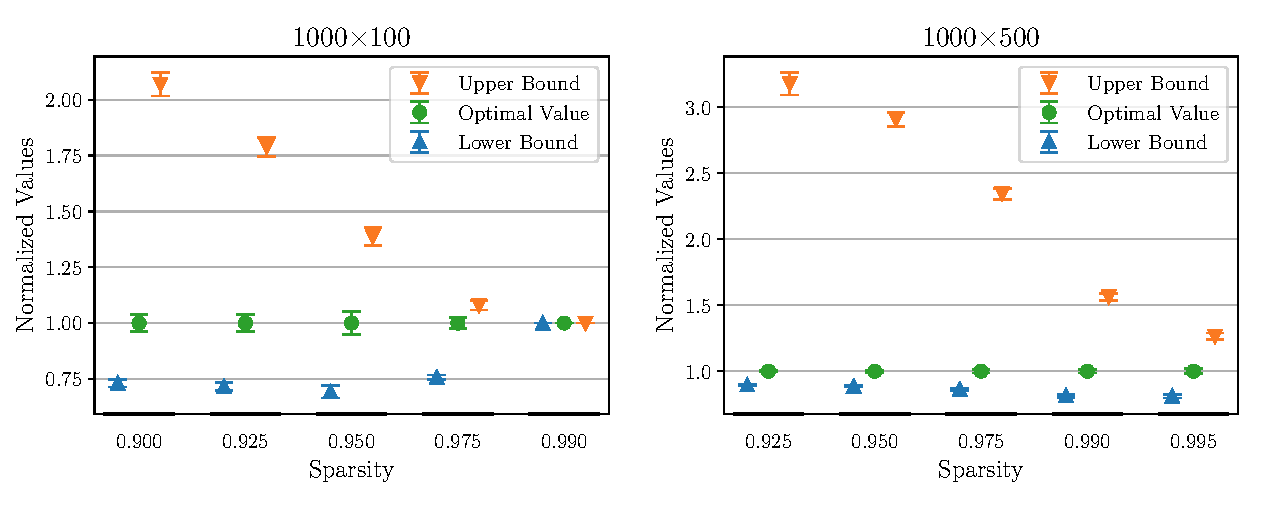
\includegraphics[width=\textwidth]{assets/figures/shape_more_vars.pdf}
    \caption{Qualità delle limitazioni prodotte dall’algoritmo di Frank-Wolfe al variare della sparsità e della forma
    della matrice di riferimento di istanze grandi.}
    \label{fig:shape3}
\end{figure}

\begin{table}[!ht]
    \centering
    \vspace*{12pt}
    \begin{tabularx}{349.48656pt}{cccc}
        \toprule
        \text{\alt Matrice} & \text{\alt Sparsità} & \text{\alt Limitazione Inferiore} & \text{\alt Limitazione Superiore} \\
        \midrule
        \( 1000\times 100 \)
        & 0.900 & 0.731 & 2.069 \\
        & 0.925 & 0.715 & 1.788 \\
        & 0.950 & 0.693 & 1.387 \\
        & 0.975 & 0.758 & 1.079 \\
        & 0.990 & 1.000 & 1.000 \\
        \midrule
        \( 1000\times 500 \)
        & 0.925 & 0.898 & 3.177 \\
        & 0.950 & 0.887 & 2.907 \\
        & 0.975 & 0.862 & 2.344 \\
        & 0.990 & 0.814 & 1.563 \\
        & 0.995 & 0.812 & 1.266 \\
        \bottomrule
    \end{tabularx}
    \caption{Valori delle limitazioni prodotte da Frank-Wolfe, normalizzati rispetto al valore ottimo fornito dal
    simplesso, al variare del bilanciamento di vincoli e variabili delle istanze.}
    \label{table:shape3}
\end{table}

In effetti, a parità di sparsità, la qualità delle limitazioni inferiori è maggiore per le matrici \( 1000\times 500 \)
piuttosto che per le matrici  \( 1000\times 100 \), nonostante la differenza nel numero totale di elementi. In aggiunta,
se confrontiamo questi risultati con quelli ottenuti in precedenza osserviamo che le matrici  \( 1000\times 1000 \)
forniscono limitazioni inferiori ancora migliori, in accordo con quanto ipotizzato.

Fino a questo momento abbiamo considerato matrici di forme differenti ma in tutti i casi il numero delle colonne era
maggiore o uguale al numero delle righe. Questa scelta deriva dal fatto che questa è la condizione più comune per le
istanze del problema del set-covering, in cui il numero dei vincoli è solitamente dominante rispetto al numero delle
variabili. Tuttavia ci sono dei contesti e delle applicazioni in cui potrebbe valere il contrario e quindi abbiamo
effettuato degli esperimenti su matrici in cui il numero delle colonne, ossia il numero di variabili, è maggiore del
numero delle righe, che rappresentano invece i vincoli. I risultati sono riassunti nei grafici della Figura
\ref{fig:shape4} e riportati nella Tabella \ref{table:shape4}.

\begin{figure}[ht]
    \centering
    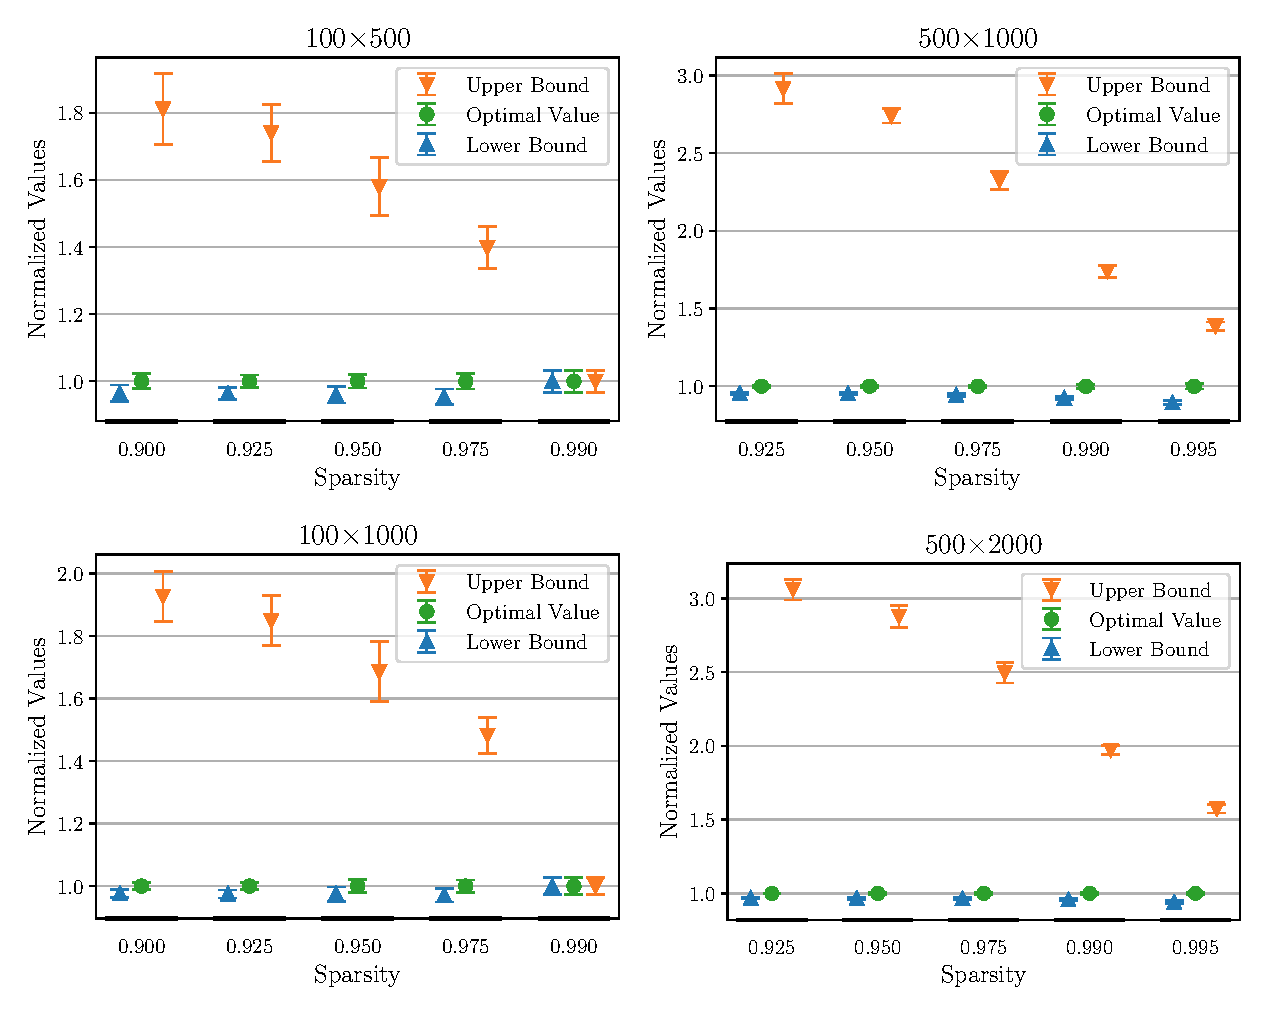
\includegraphics[width=\textwidth]{assets/figures/reverse.pdf}
    \caption{Qualità delle limitazioni prodotte dall’algoritmo di Frank-Wolfe al variare della sparsità e della forma
    della matrice di riferimento per istanze caratterizzate da un numero di variabili dominante rispetto al numero dei
    vincoli.}
    \label{fig:shape4}
\end{figure}

Osserviamo che, a parità di sparsità della matrice di riferimento e numero di vincoli dell'istanza ad essa associata,
l'aumentare del numero delle variabili è indicatore di un peggioramento nella qualità della limitazione superiore e di
un miglioramento nella qualità della limitazione inferiore. Ad esempio, le matrici \( 100\times 1000 \) producono
limitazioni inferiori migliori rispetto alle matrici \( 100\times 500 \) ma limitazioni superiori peggiori. Lo stesso
vale per le matrici \( 500\times 2000 \) e  \( 500\times 1000 \).

Se consideriamo istanze caratterizzate dallo stesso numero di variabili notiamo che, a parità di
sparsità, le limitazioni migliori si ottengono per le istanze che hanno un numero minore di vincoli. Ad esempio, le
matrici \( 100\times 1000 \) producono limitazioni migliori rispetto alle matrici \( 500\times 1000 \). Inoltre, quando
il numero delle variabili è dominante rispetto al numero dei vincoli, il bilanciamento della matrice non ha influenza
sulla qualità delle limitazioni inferiori. In realtà, le limitazioni ottenute con matrici \( 100\times 1000 \) sono
anche migliori di quelle che si ottengono con la matrice bilanciata  \( 1000\times 1000 \).


\begin{table}[!ht]
    \centering
    \vspace*{40pt}
    \begin{tabularx}{349.48656pt}{cccc}
        \toprule
        \text{\alt Matrice} & \text{\alt Sparsità} & \text{\alt Limitazione Inferiore} & \text{\alt Limitazione Superiore} \\
        \midrule
        \( 100\times 500 \)
        & 0.900 & 0.964 & 1.812 \\
        & 0.925 & 0.964 & 1.741 \\
        & 0.950 & 0.960 & 1.580 \\
        & 0.975 & 0.953 & 1.398 \\
        & 0.990 & 1.000 & 1.000 \\
        \midrule
        \( 100\times 1000 \)
        & 0.900 & 0.976 & 1.927 \\
        & 0.925 & 0.975 & 1.850 \\
        & 0.950 & 0.975 & 1.687 \\
        & 0.975 & 0.971 & 1.482 \\
        & 0.990 & 1.000 & 1.000 \\
        \midrule
        \( 500\times 1000 \)
        & 0.925 & 0.954 & 2.915 \\
        & 0.950 & 0.952 & 2.741 \\
        & 0.975 & 0.944 & 2.324 \\
        & 0.990 & 0.925 & 1.739 \\
        & 0.995 & 0.895 & 1.387 \\
        \midrule
        \( 500\times 2000 \)
        & 0.925 & 0.969 & 3.059 \\
        & 0.950 & 0.967 & 2.877 \\
        & 0.975 & 0.964 & 2.496 \\
        & 0.990 & 0.958 & 1.972 \\
        & 0.995 & 0.940 & 1.575 \\
        \bottomrule
    \end{tabularx}
    \caption{Valori delle limitazioni prodotte da Frank-Wolfe, normalizzati rispetto al valore ottimo fornito dal
    simplesso, per istanze caraterizzate da un numero di variabili dominante rispetto al numero dei vincoli.}
    \label{table:shape4}
\end{table}

Infine, se confrontiamo i risultati ottenuti con matrici caratterizzate dallo stesso numero di elementi ma con forme
simmetriche, osserviamo che le limitazioni inferiori migliori si ottengono per le matrici in cui il numero delle
variabili è dominante rispetto al numero dei vincoli, come accade ad esempio per le matrici \( 100\times 1000 \) e  \(
1000\times 1000 \) oppure \( 500\times 1000 \) e  \( 1000\times 500 \).

Per le limitazioni superiori la situazione è diversa e l'andamento sembra dipendere molto dalla sparsità della
matrice di riferimento. Per valori di sparsità abbastanza contenuti, le matrici \( 500\times 1000 \) producono
limitazioni superiori migliori, mentre quando i valori di sparsità sono più elevati le limitazioni superiori migliori
sono prodotte dalle matrici  \( 1000\times 500 \).

Di conseguenza, l'influenza della forma della matrice di riferimento delle istanze dipende dalla struttura di
quest'ultime, in quanto a numero di vincoli e di variabili.

\section{Tempi di esecuzione}
Gli esperimenti che abbiamo condotto fino a questo punto ci hanno permesso di capire come si comporta l'algoritmo di
Frank-Wolfe al variare dei parametri che identificano le istanze che abbiamo considerato, come ad esempio la sparsità,
il numero di elementi e la forma della matrice di riferimento. In particolare, abbiamo cercato di stabilire la qualità
delle limitazioni prodotte da Frank-Wolfe confrontandole con il valore ottimo ottenuto attraverso l'algoritmo del
simplesso. Analizzando i risultati che abbiamo ottenuto, siamo riusciti a concludere che la limitazione inferiore e
quella superiore si comportano in modo diverso. In particolare, la prima è molto più stabile della seconda. In generale,
abbiamo ottenuto delle limitazioni ragionevoli che richiedono ora di confrontare il tempo impiegato per ottenerle con il
tempo necessario a trovare il valore ottimo con l'algoritmo del simplesso. L'obiettivo è quello di capire se
l'algoritmo di Frank-Wolfe è in grado di produrre limitazioni di buona qualità in un tempo molto inferiore a quello
impiegato dall'algoritmo del simplesso per determinare il valore ottimo.

In questa sezione analizzeremo i tempi di esecuzione dei due algoritmi, al variare dei parametri che abbiamo
citato in precedenza. Per l'algoritmo del simplesso considereremo il tempo impiegato a trovare il valore ottimo, mentre
per l'algoritmo di Frank-Wolfe considereremo il tempo impiegato a compiere un numero di iterazioni fissato. L'idea è
quella di eseguire l'algoritmo di Frank-Wolfe molteplici volte per capire come il numero di iterazioni influenza le
limitazioni prodotte. L'obiettivo è quello di trovare un compromesso tra la qualità delle limitazioni prodotte e il
tempo impiegato per ottenerle.

\subsection{Dimensione della matrice di riferimento}
Iniziamo analizzando i risultati ottenuti dagli esperimenti svolti su istanze di dimensioni
differenti, in quanto a numero di elementi della matrice di riferimento, che sono riassunti nei grafici della Figura
\ref{fig:timesize1} e riportati nella Tabella \ref{table:timesize1}.

\begin{figure}[!ht]
    \centering
    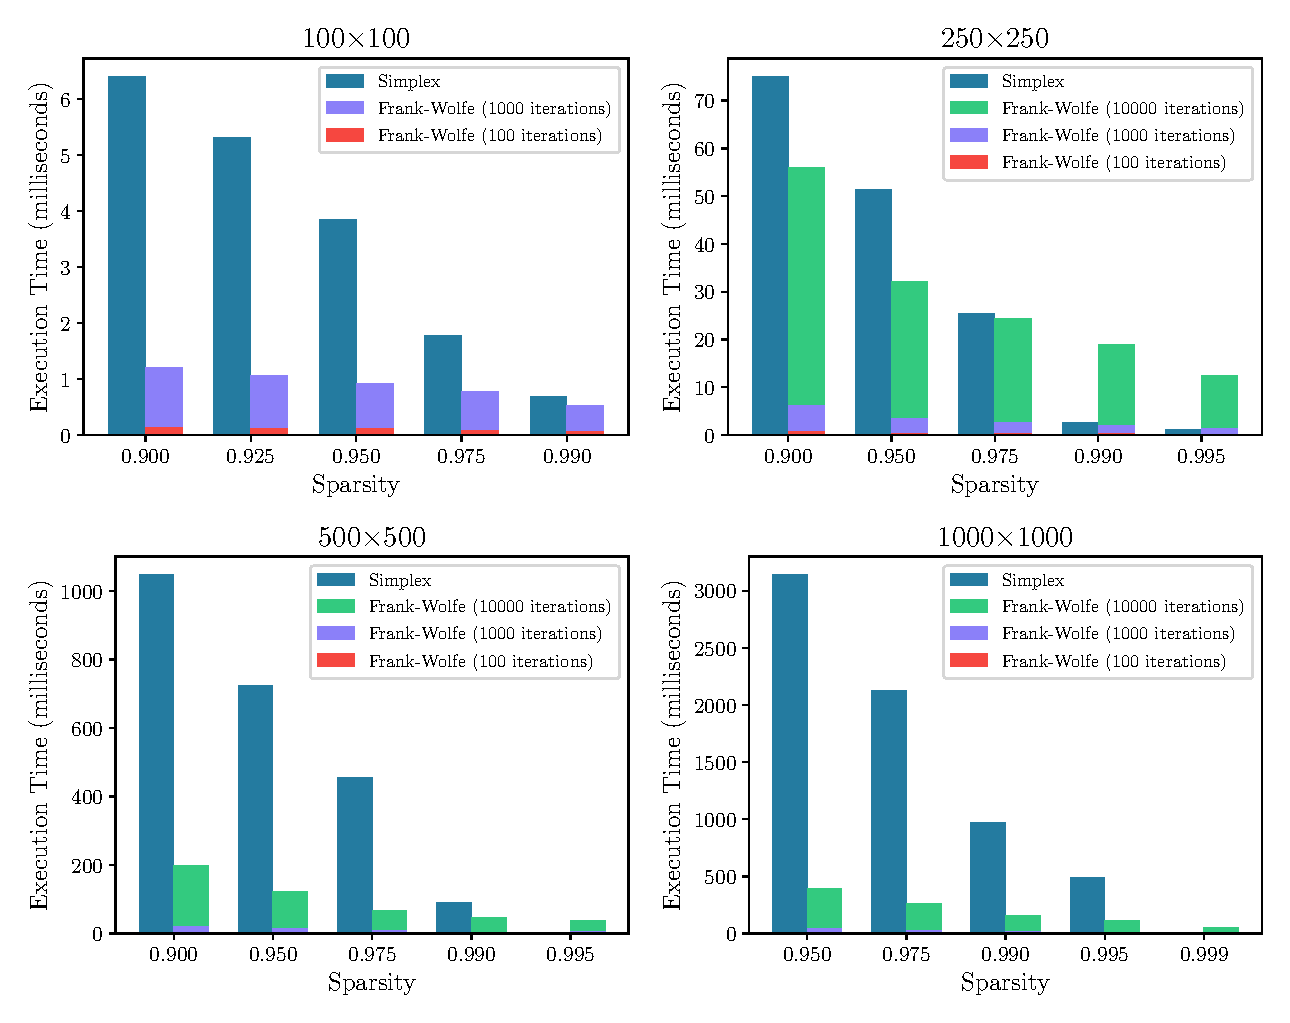
\includegraphics[width=\textwidth]{assets/figures/timesize.pdf}
    \caption{Tempi di esecuzione dell'algoritmo del simplesso e dell'algoritmo di Frank-Wolfe, al variare della sparsità
    e della dimensione della matrice di riferimento.}
    \label{fig:timesize1}
\end{figure}

In primo luogo notiamo che la sparsità della matrice ha un'influenza significativa sul tempo di esecuzione
dell'algoritmo del simplesso, soprattutto per le matrici più grandi. In particolare, l'aumento della sparsità è
indicatore di una diminuzione nel tempo di esecuzione. Per l'algoritmo di Frank-Wolfe l'effetto è il medesimo, ma è meno
marcato. Questi risultati non sono una sorpresa, poichè una matrice più sparsa richiede un numero inferiore di
operazioni da eseguire rispetto ad una matrice che ha un valore di sparsità minore.

Per istanze caratterizzate da matrici di riferimento abbastanza piccole, i tempi di esecuzione di entrambi gli algoritmi
sono molto bassi e quindi c'è poco spazio per le variazioni. Tuttavia, quando la matrice di riferimento è
sufficientemente grande, osserviamo proprio una soglia di sparsità oltre la quale l'algoritmo del simplesso è
notevolmente più veloce. L'andamento dei tempi di esecuzione dell'algoritmo di Frank-Wolfe è invece molto più stabile.

Il numero di iterazioni effettuate dall'algoritmo di Frank-Wolfe ha un'influenza significativa sul suo tempo di
esecuzione. Per questo motivo, in diverse situazioni la competitività dell'algoritmo è vincolata alla scelta di un
numero differente di iterazioni. Per le matrici più piccole, l'algoritmo del simplesso è molto veloce a prescindere dal
valore di sparsità e quindi l'algoritmo di Frank-Wolfe è competitivo solo quando il numero delle iterazioni è
contenuto. Quando le matrici sono più grandi, la sparsità gioca un ruolo fondamentale. Per valori di sparsità contenuti,
l'algoritmo del simplesso fa molta fatica e Frank-Wolfe rimane competitivo anche quando il numero delle iterazioni è
elevato.
Per valori di sparsità sufficientemente elevati, l'algoritmo del simplesso si velocizza notevolmente e Frank-Wolfe
rimane competitivo solo quando il numero delle iterazioni è abbastanza ridotto.

Nelle situazioni in cui Frank-Wolfe riesce a chiudere sul valore ottimo, tipicamente per valori di sparsità elevati, il
numero delle iterazioni necessarie è spesso molto basso e questo permette di ottenere tempi inferiori rispetto
all'algoritmo del simplesso.

In aggiunta, notiamo che per le matrici di dimensione fissata quando la sparsità aumenta il
miglioramento nella qualità delle limitazioni prodotte da Frank-Wolfe diminuisce all'aumentare del numero di iterazioni
effettuate. In altre parole, il miglioramento della qualità delle limitazioni ottenuto nel passaggio da 100 a 1000 iterazioni o da 1000 a 10000 è
maggiore quando la sparsità della matrice di riferimento è più bassa e minore quando la sparsità è più alta.

In tutti i casi, l'aumento del numero di iterazioni è indicatore di un miglioramento più marcato della limitazione
superiore piuttosto che della limitazione inferiore, che è invece molto più stabile. Inoltre, per tutte le istanze che
abbiamo considerato, il passaggio da 1000 a 10000 iterazioni determina un miglioramento trascurabile rispetto al
passaggio da 100 a 1000, soprattutto per le limitazioni inferiori delle matrici più piccole o delle matrici che hanno
valori di sparsità abbastanza elevati. Di conseguenza, molto spesso l'esecuzione di Frank-Wolfe può essere limitata a
1000 iterazioni o poco più, per ottenere limitazioni ragionevoli in tempi molto ridotti. In alcuni casi, si può andare
anche oltre e limitare il numero di iterazioni ancora di più. Le limitazioni ottenute sono comunque buone ma i tempi di
esecuzione sono di molto inferiori, soprattutto per matrici più grandi.

Negli esperimenti non abbiamo considerato esecuzioni con un numero di iterazioni più elevato di 10000 semplicemente
perché i tempi di esecuzione aumentavano troppo e il miglioramento della qualità delle limitazioni era trascurabile,
soprattutto quello della limitazione inferiore. Utilizzare un numero di iterazioni maggiore di 10000 significa perdere
la competitività dell'algoritmo di Frank-Wolfe praticamente per tutte le istanze considerate, senza però guadagnare
nulla in termini di qualità delle limitazioni.

In conclusione, l'algoritmo di Frank-Wolfe può essere competitivo indipendentemente dal numero di elementi della matrice
di riferimento, a patto di scegliere il giusto numero di iterazioni e di accontentarsi di una limitazione inferiore
buona e di una limitazione superiore discreta. Nelle situazioni in cui Frank-Wolfe è molto più veloce del simplesso, si
può considerare di aumentare il numero delle iterazioni effettuate per ottenere un miglioramento delle limitazioni,
soprattutto quella superiore, a patto di mantenere un tempo di esecuzione ridotto che garantisca la competitività con
l'algoritmo del simplesso.

\begin{landscape}
\begin{table}[!h]
    \centering
    \vspace*{30pt}
    \begin{tabularx}{665.19638pt}{cccccccccccc}
        \toprule
        & &  \multicolumn{3}{c}{\text{\alt Limitazione Inferiore}} & \multicolumn{3}{c}{\text{\alt Limitazione
Superiore}} & \multicolumn{3}{c}{\text{\alt Tempo Frank-Wolfe (ms)}}\\
        \cmidrule(lr){3-5}
        \cmidrule(lr){6-8}
        \cmidrule(lr){9-11}
        \text{\alt Matrice} & \text{\alt Sparsità} & \text{\alt 100} & \text{\alt 1000} & \text{\alt 10000} & \text{\alt 100} & \text{\alt 1000} &
        \text{\alt 10000} &
        \text{\alt 100} & \text{\alt 1000} & \text{\alt 10000} & \text{\alt Tempo Simplesso (ms)} \\
        \midrule
        \( 100\times 100 \)
        & 0.900 & 0.8576 & 0.8865 & 0.8879 & 1.9539 & 1.6905 & 1.5373 & 0.1361 & 1.2024 & 11.6732 & 6.4107 \\
        & 0.925 & 0.8576 & 0.8770 & 0.8791 & 1.7043 & 1.5328 & 1.4383 & 0.1225 & 1.0606 & 10.2862 & 5.3249 \\
        & 0.950 & 0.8409 & 0.8542 & 0.8554 & 1.4336 & 1.3292 & 1.2457 & 0.1098 & 0.9214 & 8.9731 & 3.8551 \\
        & 0.975 & 0.8598 & 0.8662 & 0.8666 & 1.1801 & 1.1163 & 1.1004 & 0.0880 & 0.7726 & 7.5559 & 1.7747 \\
        & 0.990 & 1.0000 & 1.0000 & 1.0000 & 1.0000 & 1.0000 & 1.0000 & 0.0574 & 0.5323 & 5.0913 & 0.6971 \\
        \midrule
        \( 250\times 250 \)
        & 0.900 & 0.8581 & 0.9096 & 0.9158 & 2.9567 & 2.4843 & 2.3332 & 0.7376 & 6.2793 & 55.9291 & 75.1152 \\
        & 0.950 & 0.8618 & 0.8948 & 0.8985 & 2.2658 & 2.0222 & 1.9267 & 0.3853 & 3.4301 & 32.2335 & 51.4708 \\
        & 0.975 & 0.8483 & 0.8657 & 0.8673 & 1.7121 & 1.5571 & 1.5112 & 0.2968 & 2.5420 & 24.4083 & 25.4179 \\
        & 0.990 & 0.8541 & 0.8601 & 0.8606 & 1.2323 & 1.1907 & 1.1579 & 0.2333 & 1.9958 & 18.9113 & 2.5394 \\
        & 0.995 & 1.0000 & 1.0000 & 1.0000 & 1.0000 & 1.0000 & 1.0000 & 0.1462 & 1.3031 & 12.4242 & 1.2011 \\
        \midrule
        \( 500\times 500 \)
        & 0.900 & 0.8400 & 0.9204 & 0.9299 & 3.7099 & 3.2344 & 3.0214 & 2.2067 & 20.5444 & 198.6950 & 1048.5477 \\
        & 0.950 & 0.8538 & 0.9127 & 0.9191 & 3.1156 & 2.7492 & 2.6017 & 1.4827 & 13.4749 & 121.3727 & 724.4617 \\
        & 0.975 & 0.8648 & 0.8989 & 0.9027 & 2.3895 & 2.1962 & 2.1019 & 0.8559 & 7.5704 & 67.7478 & 456.2471 \\
        & 0.990 & 0.8434 & 0.8579 & 0.8594 & 1.6196 & 1.5337 & 1.4915 & 0.6744 & 4.0800 & 46.5179 & 90.1103 \\
        & 0.995 & 0.8531 & 0.8595 & 0.8602 & 1.2834 & 1.2430 & 1.2142 & 0.4950 & 4.2763 & 38.8078 & 3.5712 \\
        \midrule
        \( 1000\times 1000 \)
        & 0.950 & 0.8346 & 0.9215 & 0.9312 & 3.8963 & 3.5183 & 3.3231 & 4.4801 & 41.5427 & 396.8238 & 3142.2952 \\
        & 0.975 & 0.8553 & 0.9131 & 0.9195 & 3.2182 & 2.9260 & 2.8220 & 3.0410 & 28.8782 & 264.5643 & 2125.8350 \\
        & 0.990 & 0.8621 & 0.8925 & 0.8957 & 2.2202 & 2.0965 & 2.0417 & 1.8980 & 17.1971 & 158.7026 & 975.0234 \\
        & 0.995 & 0.8429 & 0.8571 & 0.8585 & 1.6542 & 1.5738 & 1.5479 & 1.3779 & 12.2042 & 111.4531 & 489.7301 \\
        & 0.999 & 1.0000 & 1.0000 & 1.0000 & 1.0000 & 1.0000 & 1.0000 & 0.6364 & 5.7191 & 51.2325 & 3.6620 \\
        \bottomrule
    \end{tabularx}
    \caption{Qualità delle limitazioni (valori normalizzati rispetto all'ottimo ottenuto con l'algoritmo del simplesso)
    di Frank-Wolfe e tempo di esecuzione impiegato per ottenerle, al variare del numero di iterazioni.}
    \label{table:timesize1}
\end{table}
\end{landscape}

\subsection{Forma della matrice di riferimento}

Procediamo ora con l'analisi dei risultati ottenuti considerando istanze caratterizzate da matrici di riferimento di
forme differenti. Iniziamo considerando matrici di riferimento caratterizzate dallo stesso numero di elementi. I
risultati relativi a istanze di taglia piccola e media sono riassunti nei grafici della figura \ref{fig:timeshape} e
riportati nella tabella \ref{table:hugetable2}, mentre quelli che riguardano le istanze di taglia grande sono riassunti
nella figura \ref{fig:timeshape2} e riportati nella tabella \ref{table:hugetable3}.

\begin{figure}[!ht]
    \centering
    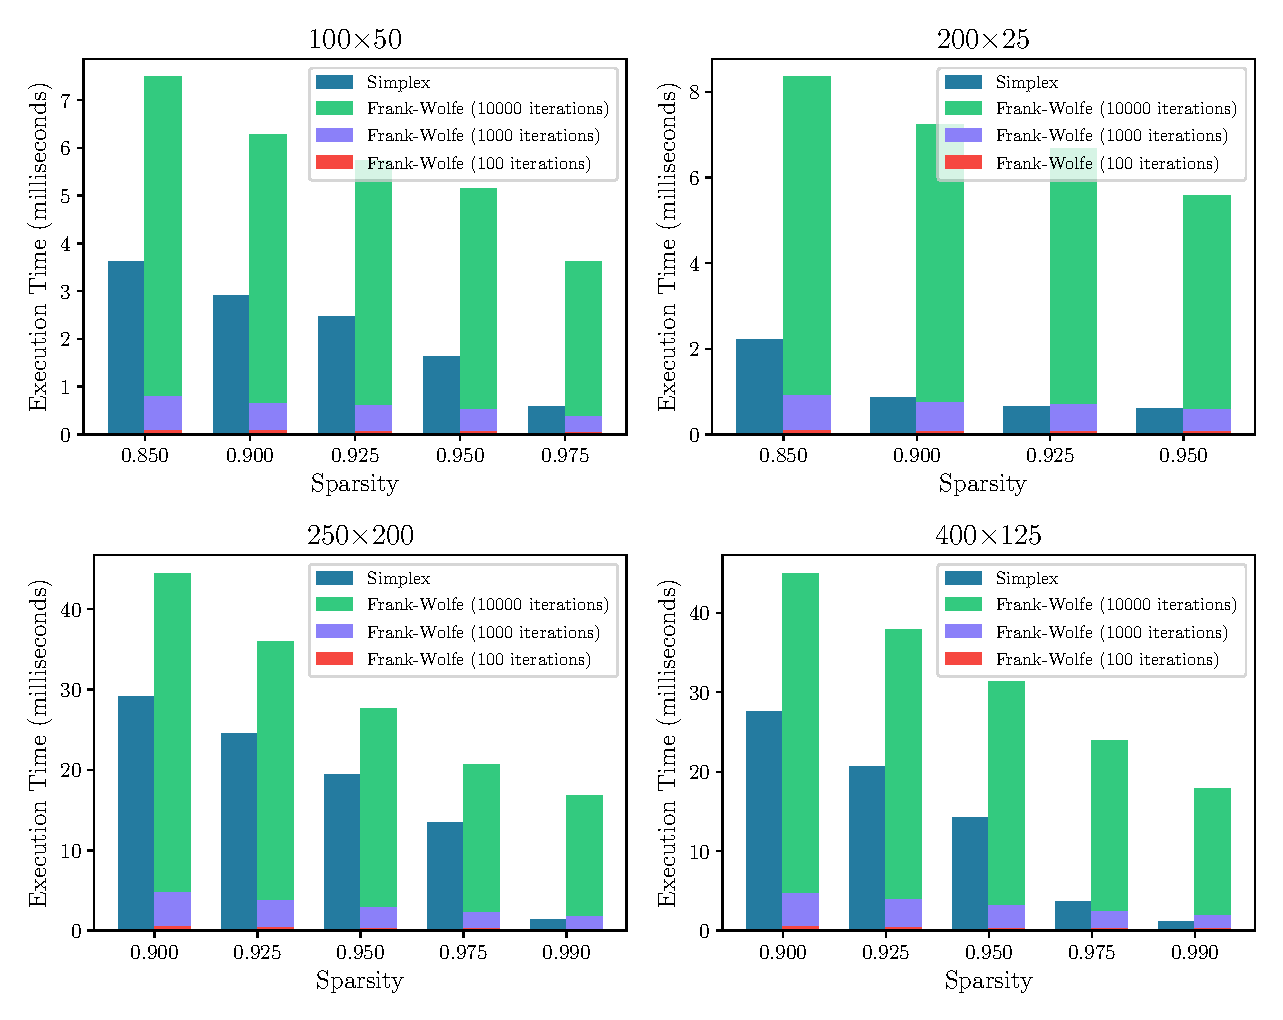
\includegraphics[width=\textwidth]{assets/figures/timeshape.pdf}
    \caption{tempo di esecuzione dell'algoritmo del simplesso e dell'algoritmo di Frank-Wolfe per istanze di taglia
    piccola e media, al variare della sparsità e della forma della matrice di riferimento.}
    \label{fig:timeshape}
\end{figure}

Per le istanze di taglia piccola, a parità di sparsità e di numero di elementi della matrice di riferimento, variare la
forma influenza in modo significativo i tempi di esecuzione dell'algoritmo del simplesso ma non quelli relativi
all'algoritmo di Frank-Wolfe, che rimangono invece molto più stabili. La variazione dei tempi di esecuzione
dell'algoritmo del simplesso è particolarmente evidente quando i valori di sparsità sono elevati. In particolare,
l'algoritmo del simplesso impiega meno tempo a risolvere le istanze che hanno un numero minore di variabili. Ad esempio,
il tempo impiegato per risolvere le istanze \( 200\times 25 \) è mediamente inferiore a quello necessario per risolvere
le istanze  \( 100\times 50 \), nonostante il numero degli elementi sia lo stesso. Lo stesso vale per le matrici \(
250\times 200 \) e  \( 400\times 125 \), anche se l'effetto è meno marcato, soprattuto per i valori di sparsità più
bassi.

\begin{figure}[!ht]
    \centering
    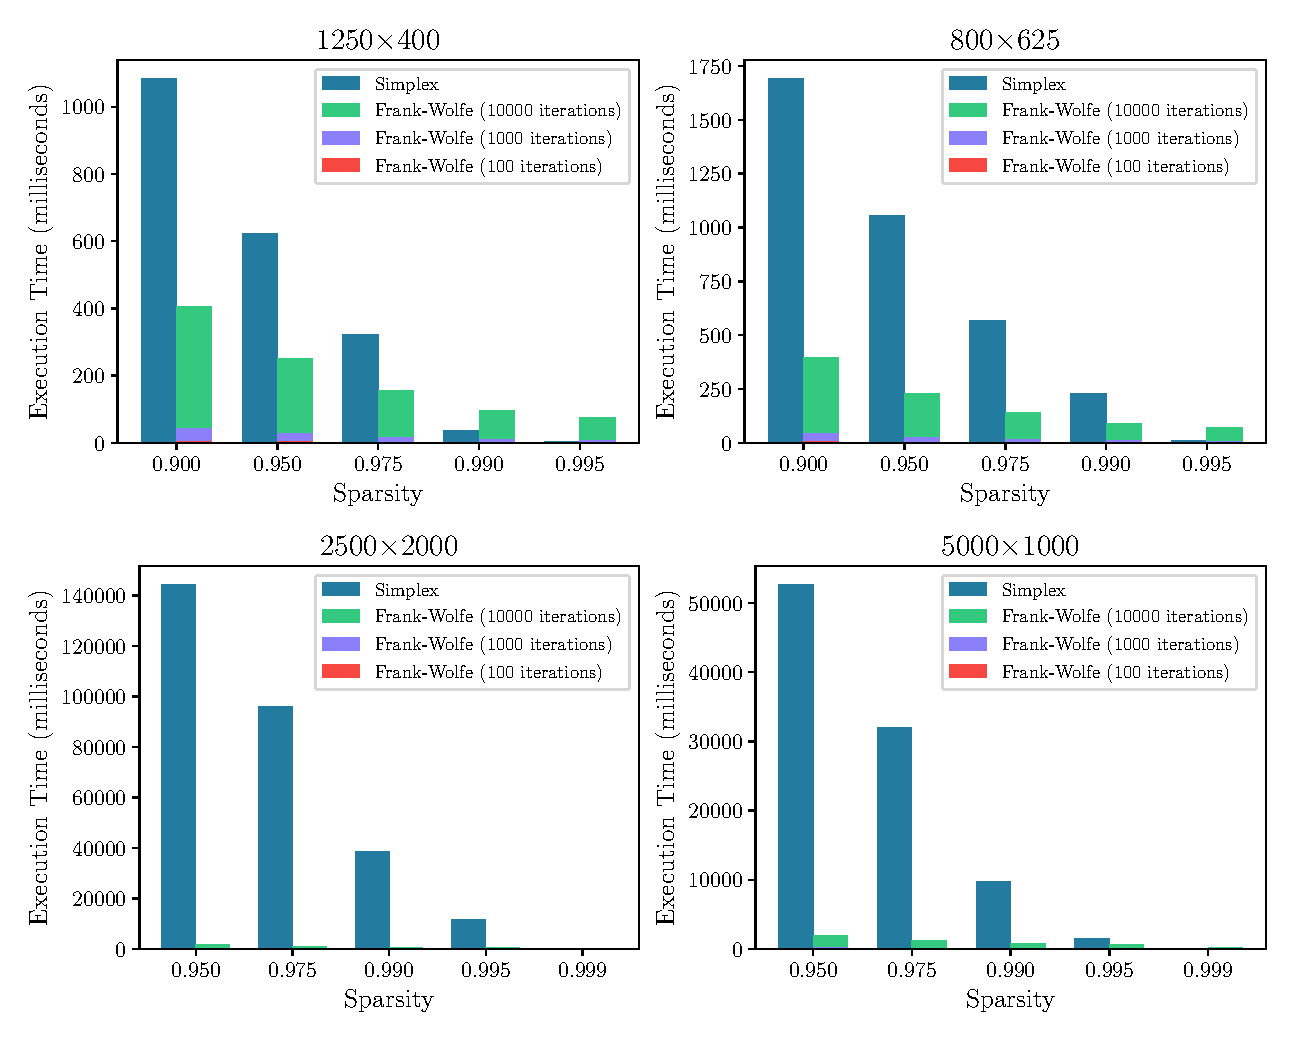
\includegraphics[width=\textwidth]{assets/figures/timeshape2.pdf}
    \caption{tempo di esecuzione dell'algoritmo del simplesso e dell'algoritmo di Frank-Wolfe per istanze di taglia
    grande, al variare della sparsità e della forma della matrice di riferimento.}
    \label{fig:timeshape2}
\end{figure}

Per le matrici più grandi, il comportamento è lo stesso ma è più marcato. In particolare, i tempi dell'algoritmo del
simplesso variano notevolmente a seconda della forma della matrice di riferimento. Ad esempio, per le matrici \(
2500\times 2000 \) e \( 5000\times 1000\), i tempi di esecuzione sono molto differenti. L'effetto è uguale ma meno
marcato per le matrici \( 800\times 625 \) e \( 1250\times 400 \). Di conseguenza, più è grande la matrice, e maggiore
sarà l'influenza della sua forma sui tempi di esecuzione dell'algoritmo del simplesso. Anche in questo caso, l'algoritmo
di Frank-Wolfe ha tempi molto più stabili. Inoltre, i tempi di Frank-Wolfe sono così ridotti rispetto a quelli del
simplesso che per matrici sufficientemente grandi non sono neanche visibili nei grafici. In questi casi l'algoritmo di
Frank-Wolfe riesce comunque a trovare delle buone limitazioni, con il vantaggio di impiegare molto meno tempo rispetto
all'algoritmo del simplesso.

Infine, consideriamo le istanze caratterizzate da matrici di riferimento simmetriche, i cui risultati sono riassunti nei
grafici della Figura \ref{fig:timeshapelast} e riportati nella tabella \ref{table:hugetable4}.

\begin{figure}[!ht]
    \centering
    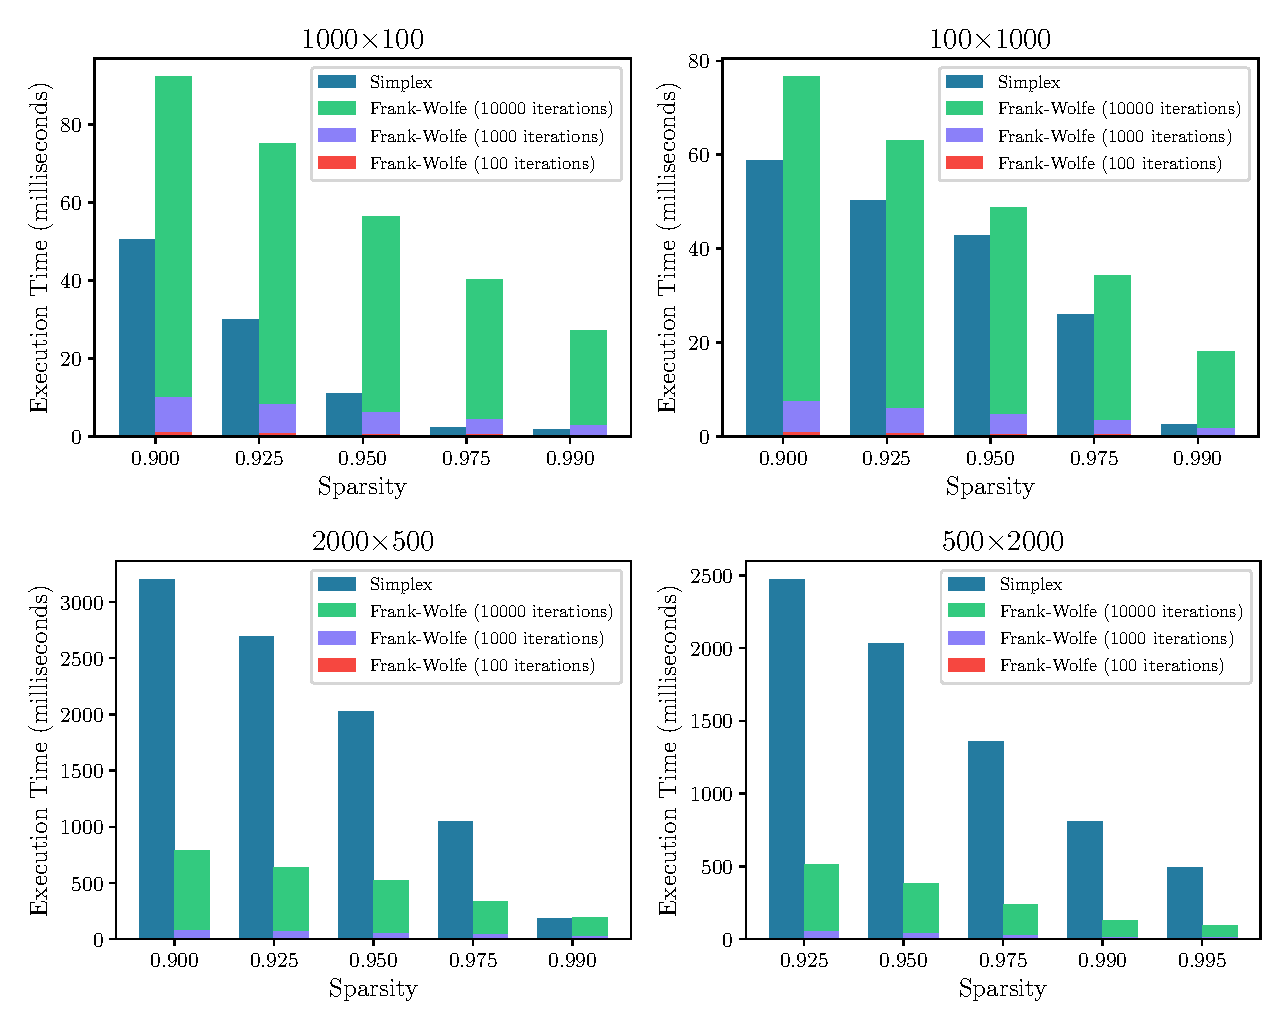
\includegraphics[width=\textwidth]{assets/figures/symmetricshape.pdf}
    \caption{tempo di esecuzione dell'algoritmo del simplesso e dell'algoritmo di Frank-Wolfe per istanze di taglia
    grande, al variare della sparsità e della forma della matrice di riferimento.}
    \label{fig:timeshapelast}
\end{figure}

Osserviamo che i tempi di esecuzione dell'algoritmo di Frank-Wolfe sono migliori per le matrici che hanno un numero di
variabili dominante rispetto al numero dei vincoli, mentre l'algoritmo del simplesso ha invece un comportamento più
irregolare.

\begin{landscape}
\begin{table}[!h]
    \centering
    \vspace*{30pt}
    \begin{tabularx}{641.68651pt}{cccccccccccc}
        \toprule
        & &  \multicolumn{3}{c}{\text{\alt Limitazione Inferiore}} & \multicolumn{3}{c}{\text{\alt Limitazione
Superiore}} & \multicolumn{3}{c}{\text{\alt Tempo Frank-Wolfe (ms)}}\\
        \cmidrule(lr){3-5}
        \cmidrule(lr){6-8}
        \cmidrule(lr){9-11}
        \text{\alt Matrice} & \text{\alt Sparsità} & \text{\alt 100} & \text{\alt 1000} & \text{\alt 10000} & \text{\alt 100} & \text{\alt 1000} &
        \text{\alt 10000} &
        \text{\alt 100} & \text{\alt 1000} & \text{\alt 10000} & \text{\alt Tempo Simplesso (ms)} \\
        \midrule
        \( 100\times 50 \)
        & 0.850 & 0.8075 & 0.8300 & 0.8321 & 1.7883 & 1.5568 & 1.4179 & 0.0893 & 0.8044 & 7.4851 & 3.6191 \\
        & 0.900 & 0.8004 & 0.8148 & 0.8159 & 1.4754 & 1.3387 & 1.2667 & 0.0811 & 0.6531 & 6.2725 & 2.8984 \\
        & 0.925 & 0.7909 & 0.8008 & 0.8018 & 1.2999 & 1.1949 & 1.1581 & 0.0682 & 0.5996 & 5.7267 & 2.4767 \\
        & 0.950 & 0.8122 & 0.8201 & 0.8206 & 1.1685 & 1.0866 & 1.0625 & 0.0607 & 0.5266 & 5.1577 & 1.6346 \\
        & 0.975 & 0.9309 & 0.9341 & 0.9345 & 1.0207 & 1.0109 & 1.0109 & 0.0455 & 0.3835 & 3.6199 & 0.5816 \\
        \midrule
        \( 200\times 25 \)
        & 0.850 & 0.6809 & 0.6981 & 0.6991 & 1.2374 & 1.1422 & 1.1061 & 0.0923 & 0.9169 & 8.3504 & 2.2107 \\
        & 0.900 & 0.7347 & 0.7461 & 0.7467 & 1.0633 & 1.0173 & 1.0035 & 0.0786 & 0.7532 & 7.2365 & 0.8551 \\
        & 0.925 & 0.8204 & 0.8297 & 0.8300 & 1.0228 & 1.0021 & 1.0000 & 0.0732 & 0.6935 & 6.6782 & 0.6583 \\
        & 0.950 & 0.9466 & 0.9522 & 0.9524 & 1.0000 & 1.0000 & 1.0000 & 0.0687 & 0.5865 & 5.5813 & 0.6166 \\
        \midrule
        \( 250\times 200 \)
        & 0.900 & 0.8502 & 0.8974 & 0.9030 & 2.8143 & 2.3623 & 2.2692 & 0.5373 & 4.7315 & 44.4727 & 29.1073 \\
        & 0.925 & 0.8477 & 0.8900 & 0.8946 & 2.5181 & 2.2540 & 2.0996 & 0.4176 & 3.7669 & 35.9471 & 24.5079 \\
        & 0.950 & 0.8478 & 0.8777 & 0.8807 & 2.1247 & 1.9606 & 1.8297 & 0.3296 & 2.9376 & 27.6306 & 19.3998 \\
        & 0.975 & 0.8262 & 0.8401 & 0.8416 & 1.5418 & 1.4524 & 1.3977 & 0.2566 & 2.2062 & 20.6300 & 13.4564 \\
        & 0.990 & 0.8658 & 0.8699 & 0.8706 & 1.1950 & 1.1459 & 1.1137 & 0.2027 & 1.7696 & 16.8272 & 1.4226 \\
        \midrule
        \( 400\times 125 \)
        & 0.900 & 0.7740 & 0.8207 & 0.8251 & 2.5543 & 2.3076 & 2.2024 & 0.5037 & 4.6682 & 44.9879 & 27.5289 \\
        & 0.925 & 0.7712 & 0.8106 & 0.8134 & 2.2316 & 2.0595 & 1.9619 & 0.4126 & 3.9644 & 37.8337 & 20.6659 \\
        & 0.950 & 0.7666 & 0.7891 & 0.7904 & 1.8273 & 1.6992 & 1.6352 & 0.3409 & 3.2158 & 31.3210 & 14.1838 \\
        & 0.975 & 0.7541 & 0.7667 & 0.7677 & 1.3465 & 1.2681 & 1.2408 & 0.2768 & 2.4524 & 23.9097 & 3.6768 \\
        & 0.990 & 0.9168 & 0.9208 & 0.9213 & 1.0490 & 1.0490 & 1.0490 & 0.2201 & 1.8997 & 17.8531 & 1.1396 \\
        \bottomrule
    \end{tabularx}
    \caption{qualità delle limitazioni (valori normalizzati rispetto all'ottimo ottenuto con l'algoritmo del simplesso)
    di Frank-Wolfe e tempo di esecuzione impiegato per ottenerle, al variare del numero di iterazioni e della forma
    della matrice di riferimento.}
    \label{table:hugetable2}
\end{table}
\end{landscape}

\begin{landscape}
\begin{table}[!h]
    \centering
    \vspace*{30pt}
    \begin{tabularx}{677.40169pt}{cccccccccccc}
        \toprule
        & &  \multicolumn{3}{c}{\text{\alt Limitazione Inferiore}} & \multicolumn{3}{c}{\text{\alt Limitazione
Superiore}} & \multicolumn{3}{c}{\text{\alt Tempo Frank-Wolfe (ms)}}\\
        \cmidrule(lr){3-5}
        \cmidrule(lr){6-8}
        \cmidrule(lr){9-11}
        \text{\alt Matrice} & \text{\alt Sparsità} & \text{\alt 100} & \text{\alt 1000} & \text{\alt 10000} & \text{\alt 100} & \text{\alt 1000} &
        \text{\alt 10000} &
        \text{\alt 100} & \text{\alt 1000} & \text{\alt 10000} & \text{\alt Rempo Simplesso (ms)} \\
        \midrule
        \( 800\times 625 \)
        & 0.900 & 0.8184 & 0.9150 & 0.9270 & 4.1312 & 3.6840 & 3.4339 & 4.5415 & 44.5577 & 395.634 & 1693.215 \\
        & 0.950 & 0.8327 & 0.9037 & 0.9115 & 3.4963 & 3.1305 & 2.9875 & 2.5951 & 26.1331 & 230.076 & 1057.753 \\
        & 0.975 & 0.8444 & 0.8912 & 0.8961 & 2.7755 & 2.5332 & 2.4472 & 1.6854 & 15.1159 & 140.394 & 566.465 \\
        & 0.990 & 0.8361 & 0.8559 & 0.8576 & 1.8471 & 1.7506 & 1.7032 & 1.1039 & 9.7862 & 91.465 & 228.820 \\
        & 0.995 & 0.8247 & 0.8335 & 0.8345 & 1.4170 & 1.3630 & 1.3357 & 0.8481 & 7.4766 & 69.661 & 12.075 \\
        \midrule
        \( 1250\times 400 \)
        & 0.900 & 0.7559 & 0.8695 & 0.8806 & 4.1034 & 3.7554 & 3.5263 & 4.4671 & 43.4733 & 406.711 & 1084.810 \\
        & 0.950 & 0.7756 & 0.8451 & 0.8519 & 3.3665 & 3.0883 & 2.9520 & 2.7899 & 27.3705 & 252.102 & 621.661 \\
        & 0.975 & 0.7768 & 0.8156 & 0.8198 & 2.4684 & 2.3355 & 2.2635 & 1.7517 & 16.4673 & 155.664 & 321.928 \\
        & 0.990 & 0.7536 & 0.7690 & 0.7704 & 1.5636 & 1.5005 & 1.4694 & 1.1264 & 10.4208 & 97.371 & 37.720 \\
        & 0.995 & 0.8002 & 0.8088 & 0.8097 & 1.2343 & 1.2343 & 1.2328 & 0.8521 & 7.8722 & 74.626 & 3.426 \\
        \midrule
        \( 2500\times 2000 \)
        & 0.950 & 0.7961 & 0.9216 & 0.9372 & 5.1203 & 4.5322 & 4.2721 & 18.7118 & 178.5077 & 1770.390 & 144365.114 \\
        & 0.975 & 0.8211 & 0.9139 & 0.9245 & 4.2592 & 3.8775 & 3.6957 & 11.3902 & 103.9968 & 1022.290 & 95927.598 \\
        & 0.990 & 0.8420 & 0.8985 & 0.9044 & 3.1200 & 2.9310 & 2.8412 & 6.8700 & 62.3454 & 608.851 & 38566.928 \\
        & 0.995 & 0.8478 & 0.8821 & 0.8855 & 2.3680 & 2.2480 & 2.2067 & 5.3173 & 48.9663 & 471.568 & 11814.630 \\
        & 0.999 & 0.8654 & 0.8707 & 0.8713 & 1.2712 & 1.2583 & 1.2427 & 2.8082 & 25.5904 & 237.038 & 9.312 \\
        \midrule
        \( 5000\times 1000 \)
        & 0.950 & 0.7182 & 0.8530 & 0.8674 & 4.9974 & 4.5726 & 4.4043 & 20.5998 & 197.0393 & 1911.559 & 52680.412 \\
        & 0.975 & 0.7409 & 0.8262 & 0.8347 & 3.9821 & 3.7235 & 3.6208 & 13.0027 & 121.8646 & 1239.010 & 32048.006 \\
        & 0.990 & 0.7378 & 0.7818 & 0.7858 & 2.5930 & 2.5263 & 2.4800 & 8.6056 & 80.4950 & 761.756 & 9718.694 \\
        & 0.995 & 0.7253 & 0.7464 & 0.7482 & 1.7859 & 1.7366 & 1.7041 & 6.6523 & 61.8239 & 586.782 & 1440.216 \\
        & 0.999 & 1.0000 & 1.0000 & 1.0000 & 1.0000 & 1.0000 & 1.0000 & 2.0833 & 19.2386 & 168.014 & 7.510 \\
        \bottomrule
    \end{tabularx}
    \caption{qualità delle limitazioni (valori normalizzati rispetto all'ottimo ottenuto con l'algoritmo del simplesso)
    di Frank-Wolfe e tempo di esecuzione impiegato per ottenerle, al variare del numero di iterazioni e della forma
    della matrice di riferimento.}
    \label{table:hugetable3}
\end{table}
\end{landscape}

\begin{landscape}
\begin{table}[!h]
    \centering
    \vspace*{30pt}
    \begin{tabularx}{659.32144pt}{cccccccccccc}
        \toprule
        & &  \multicolumn{3}{c}{\text{\alt Limitazione Inferiore}} & \multicolumn{3}{c}{\text{\alt Limitazione
Superiore}} & \multicolumn{3}{c}{\text{\alt Tempo Frank-Wolfe (ms)}}\\
        \cmidrule(lr){3-5}
        \cmidrule(lr){6-8}
        \cmidrule(lr){9-11}
        \text{\alt Matrice} & \text{\alt Sparsità} & \text{\alt 100} & \text{\alt 1000} & \text{\alt 10000} & \text{\alt 100} & \text{\alt 1000} &
        \text{\alt 10000} &
        \text{\alt 100} & \text{\alt 1000} & \text{\alt 10000} & \text{\alt Tempo Simplesso (ms)} \\
        \midrule
        \( 1000\times 100 \)
        & 0.900 & 0.6838 & 0.7278 & 0.7309 & 2.4425 & 2.2732 & 2.1281 & 1.0560 & 10.1338 & 92.2318 & 50.4139 \\
        & 0.925 & 0.6804 & 0.7122 & 0.7146 & 2.0360 & 1.9230 & 1.8369 & 0.8351 & 8.1567 & 74.9928 & 30.0877 \\
        & 0.950 & 0.6692 & 0.6912 & 0.6927 & 1.5582 & 1.4778 & 1.4341 & 0.6365 & 6.1303 & 56.3676 & 11.0046 \\
        & 0.975 & 0.7410 & 0.7568 & 0.7575 & 1.1044 & 1.1038 & 1.0966 & 0.4589 & 4.3189 & 40.2606 & 2.2546 \\
        & 0.990 & 1.0000 & 1.0000 & 1.0000 & 1.0000 & 1.0000 & 1.0000 & 0.3146 & 2.9617 & 27.2564 & 1.8022 \\
        \midrule
        \( 100\times 1000 \)
        & 0.900 & 0.9270 & 0.9712 & 0.9752 & 2.7050 & 2.2530 & 2.0232 & 0.8954 & 7.4488 & 76.6151 & 58.8196 \\
        & 0.925 & 0.9325 & 0.9708 & 0.9745 & 2.5234 & 2.1253 & 1.9730 & 0.7292 & 6.0458 & 63.0342 & 50.1840 \\
        & 0.950 & 0.9411 & 0.9715 & 0.9743 & 2.2981 & 1.9397 & 1.7879 & 0.5587 & 4.7717 & 48.8442 & 42.7688 \\
        & 0.975 & 0.9531 & 0.9690 & 0.9703 & 1.8491 & 1.6200 & 1.5382 & 0.3999 & 3.3857 & 34.2001 & 25.9526 \\
        & 0.990 & 1.0000 & 1.0000 & 1.0000 & 1.0000 & 1.0000 & 1.0000 & 0.1775 & 1.7352 & 18.0140 & 2.6631 \\
        \midrule
        \( 2000\times 500 \)
        & 0.900 & 0.7385 & 0.8657 & 0.8787 & 4.6149 & 4.1923 & 3.9683 & 8.1339 & 79.8394 & 788.0149 & 3203.9266 \\
        & 0.925 & 0.7417 & 0.8545 & 0.8658 & 4.2667 & 3.9206 & 3.7215 & 6.8496 & 69.1491 & 639.2950 & 2693.2720 \\
        & 0.950 & 0.7568 & 0.8387 & 0.8465 & 3.7923 & 3.4758 & 3.3291 & 5.2936 & 50.9565 & 519.3931 & 2027.2962 \\
        & 0.975 & 0.7568 & 0.8098 & 0.8145 & 2.8693 & 2.6947 & 2.6113 & 3.6144 & 38.0744 & 336.7734 & 1045.2121 \\
        & 0.990 & 0.7432 & 0.7635 & 0.7652 & 1.7597 & 1.6977 & 1.6525 & 2.1082 & 20.1108 & 188.2672 & 187.5982 \\
        \midrule
        \( 500\times 2000 \)
        & 0.925 & 0.8667 & 0.9579 & 0.9679 & 4.1039 & 3.4251 & 3.1738 & 5.3659 & 51.5759 & 512.6423 & 2473.6085 \\
        & 0.950 & 0.8836 & 0.9583 & 0.9662 & 3.7045 & 3.1601 & 3.0080 & 3.9270 & 38.4495 & 379.7790 & 2030.5913 \\
        & 0.975 & 0.9061 & 0.9578 & 0.9635 & 3.0555 & 2.7320 & 2.5654 & 2.5957 & 23.9551 & 239.8961 & 1358.5758 \\
        & 0.990 & 0.9272 & 0.9552 & 0.9581 & 2.2804 & 2.0995 & 2.0162 & 1.5630 & 12.9429 & 129.9060 & 807.6202 \\
        & 0.995 & 0.9256 & 0.9388 & 0.9402 & 1.7528 & 1.6508 & 1.6046 & 1.2493 & 9.2556 & 95.7591 & 490.6100 \\
        \bottomrule
    \end{tabularx}
    \caption{qualità delle limitazioni (valori normalizzati rispetto all'ottimo ottenuto con l'algoritmo del simplesso)
    di Frank-Wolfe e tempo di esecuzione impiegato per ottenerle, al variare del numero di iterazioni e della forma
    della matrice di riferimento.}
    \label{table:hugetable4}
\end{table}
\end{landscape}
